\section{Operator Spreading in Time-Independent Hamiltonian Systems} \label{sec:opsp}

%Just do all intro here, and then decide later what to put into the circuit section

\subsection{Motivation: Thermalization} \label{sub:therm}

Discuss information movement in Time-Independent Hamiltonian systems
  Find a source for this
  What is the relationship between entropy and OTOC?
  Argument about extremal slope
    From Nahum: stairs to separate $v_B$ and $v_E$ - It is possible to make $v_E << v_B$ in quantum circuit architectures [CITE], which will be discussed in section~\ref{sec:circuits}
    
For now use Jonay paper, but hopefully find another. Could use Keyserlingk but it would be nice to save that for the discussion of random unitary dynamics.

Although most sources consider symmetric dynamics [CITE] this is not a requirement. Find the Nahum paper that discusses asymmetric systems.

\subsection{Background: Evolution in Time} \label{sub:evoltime}

All systems considered in this thesis will exist on spin chains, one-dimensional collection of quantum degrees of freedom. Initially we consider systems with $q=2$ degrees of freedom at each site, such as a chain of spin-$\half$ particles. Later, we will consider sites with more degrees of freedom. 

Under a time-independent Hamiltonian $H$, states of the system evolve in the Schr\"odinger picture as 
\begin{align}
\ket{\psi(t)} = U(t)\ket{\psi(0)},\quad U(t) = \e^{-iHt}. \label{eqn:shro}
\end{align}
This evolution can be generalized to a time-dependent Hamiltonian by evolving with the time-ordered unitary operator
\begin{align}
U(t,t_0) = \text{T}\e^{-i\int_{t_0}^td\tau H(\tau)}.
\end{align}
As we will consider time-independent Hamiltonians, we only need time evolution operators of the form of equation~\ref{eqn:shro}. 

Instead of evolving states, it is possible to evolve operators under the Heisenberg picture. In order to preserve the time dependence of expectation values, the operators must evolve as 
\begin{align}
A(t) = U^\dag(t)\,A(0)\,U(t) = \e^{iHt}A(0)\,\e^{-iHt}.\label{eqn:heis}
\end{align}

One remark worth making about time evolution in different pictures is that operators aren't the only the only important Hermitian matrix in the system. The density matrix $\rho$ describes the state of the system, and in pure states is $\rho = \ket{\psi}\bra{\psi}$. Density matrices are more general than kets, though, because they can represent mixed states. In the Schr\"odinger picture $\rho$ evolves the way its construction would imply
\begin{align}
\rho(t) = \e^{-iHt}\rho(0)\e^{iHt}
\end{align}
while it does not evolve in the Heisenberg picture. This is the opposite of observables, so when discussing the evolution of matrices it is necessary to specify whether they are observables or density matrices.

\subsection{Pauli Strings and Pauli Weight} \label{sub:pauli}

This subsection is based on~\cite{Keyserlingk}. Since it is possible to add Hermitian operators and multiply them by constants, they live in a vector space that can be described using some basis. When discussing operator spreading it is convenient to decompose operators that may act on very high dimensional Hilbert spaces into the Pauli basis. The basis operators are tensor products of Pauli matrices. Eventually we will decompose operators that are initially local, but any operator can be decomposed in this manner.

For single sites with Hilbert spaces of complex dimension $q$, the space of Hermitian operators is $q^2$-dimensional. For $q=2$ the basis operators are $X, Y, Z, I$. In general, there will be two Hermitian operators $X$ and $Z$ that obey $ZX = \exp(2\pi i/q)XZ$ and $Z^q=X^q=I$. Then an arbitrary basis operator will be of the form 
\begin{align}
\sigma^\mu = \phi X^{\mu_1}Z^{\mu_2},
\end{align}
where $\mu_1, \mu_2\in\{0,1,\dots,q-1\}$ and $\phi$ is a phase to preserve Hermiticity. We can extend this description to multiple sites by taking tensor products of $L$ basis operators with subscript $\nu$ representing $L$ $\mu$ indices. Under the matrix norm $||M|| = \text{tr}(M^\dag M)/q^L$, this basis is orthonormal:
\begin{align}
\th{q}\text{tr}(\sigma^{\mu\dag}\sigma^\nu) &= \th{q}\text{tr}(Z^{\mu_2\dag}
	X^{\mu_1\dag}X^{\nu_1}Z^{\nu_2})\nn
&= \delta_{\mu\nu}.\label{eqn:orthonorm}
\end{align}

A general operator $A = \sum_\nu c_{\nu}(0)\sigma^\nu$ evolves into
\begin{align}
A(t) = U^\dag(t)A\,U(t) = \sum_\nu c_\nu(t)\sigma^\nu.\label{eqn:decomp}
\end{align}
Due to the orthonormality, the coefficients are 
\begin{align}
c_\nu(t) = \th{q^L}\text{tr}(\sigma^{\nu\dag}A(t))
\end{align}
and obey 
\begin{align}
\dt \left(\sum_\nu \abs{c_\nu}^2\right) = 0 \nonumber
\end{align}
due to unitarity.

With $c_\nu(t)$ in hand, we can define the Pauli weight $W(i,t)$ as how many of the Pauli strings in the decomposition end on site $i$, weighted by their coefficients in Eq.~\ref{eqn:decomp},
\begin{align}
W(i,t) = \sum_\nu\abs{c_\nu(t)}^2\,\delta(\text{end}(\nu)=i).
	\label{eqn:endweight}
\end{align}
The delta function constrains the sum to be only over $\nu$ such that $\sigma^\nu$ has a non-identity at site $i$ and identities at all sites right of $i$. This gives a measure of how far the operator has spread. Reference~\cite{Keyserlingk} refers to this quantity as $\rho$ to emphasize its conservation and hydrodynamic evolution. It is possible to define an analogous quantity with the sum over strings that begin on site $i$ and have identities on all sites left of $i$. In that case the quantity in equation~\ref{eqn:endweight} can be called $W_R(i,t)$ while the weight of sites that start on $i$ is $W_L(i,t)$.

As an example, write
\begin{align}
A = \th{\sqrt{2}} X_0\otimes Y_1\otimes Y_2\otimes I_3 + \th{\sqrt{2}} I_0\otimes I_1\otimes Z_2\otimes Z_3,
	\nonumber
\end{align}
where the subscript designates the site on which each operator acts. This can be shortened to
\begin{align}
A = \th{\sqrt{2}} XYYI + \th{\sqrt{2}} IIZZ\label{eqn:inioper}.
\end{align}
Then the right (ending) Pauli weights are $W_R(0,0) = W_R(1,0) = 0$, $W_R(2,0)= W_R(3,0) =\half$, while the left (starting) weights are $W_L(0, 0) = W(2,0) =\half$, $W_L(1,0) = W_L(3,0)=0$.

This decomposition is particularly useful when the initial operator is local. This means that all strings in the Pauli decomposition contain non-identiy operators at a single site. Then the end weights describe how far the operator has spread throughout the system due to the unitary dynamics, which is what allows the systems to localize. Figure~\ref{fig:hamspreading} shows the Pauli end weight evolution for an initially local operator in an Ising spin chain with longitudinal field in a strongly chaotic phase~\cite{Jonay17}. The weight eventually reaches the last site after moving across all sites.

\begin{figure}
	\centering
	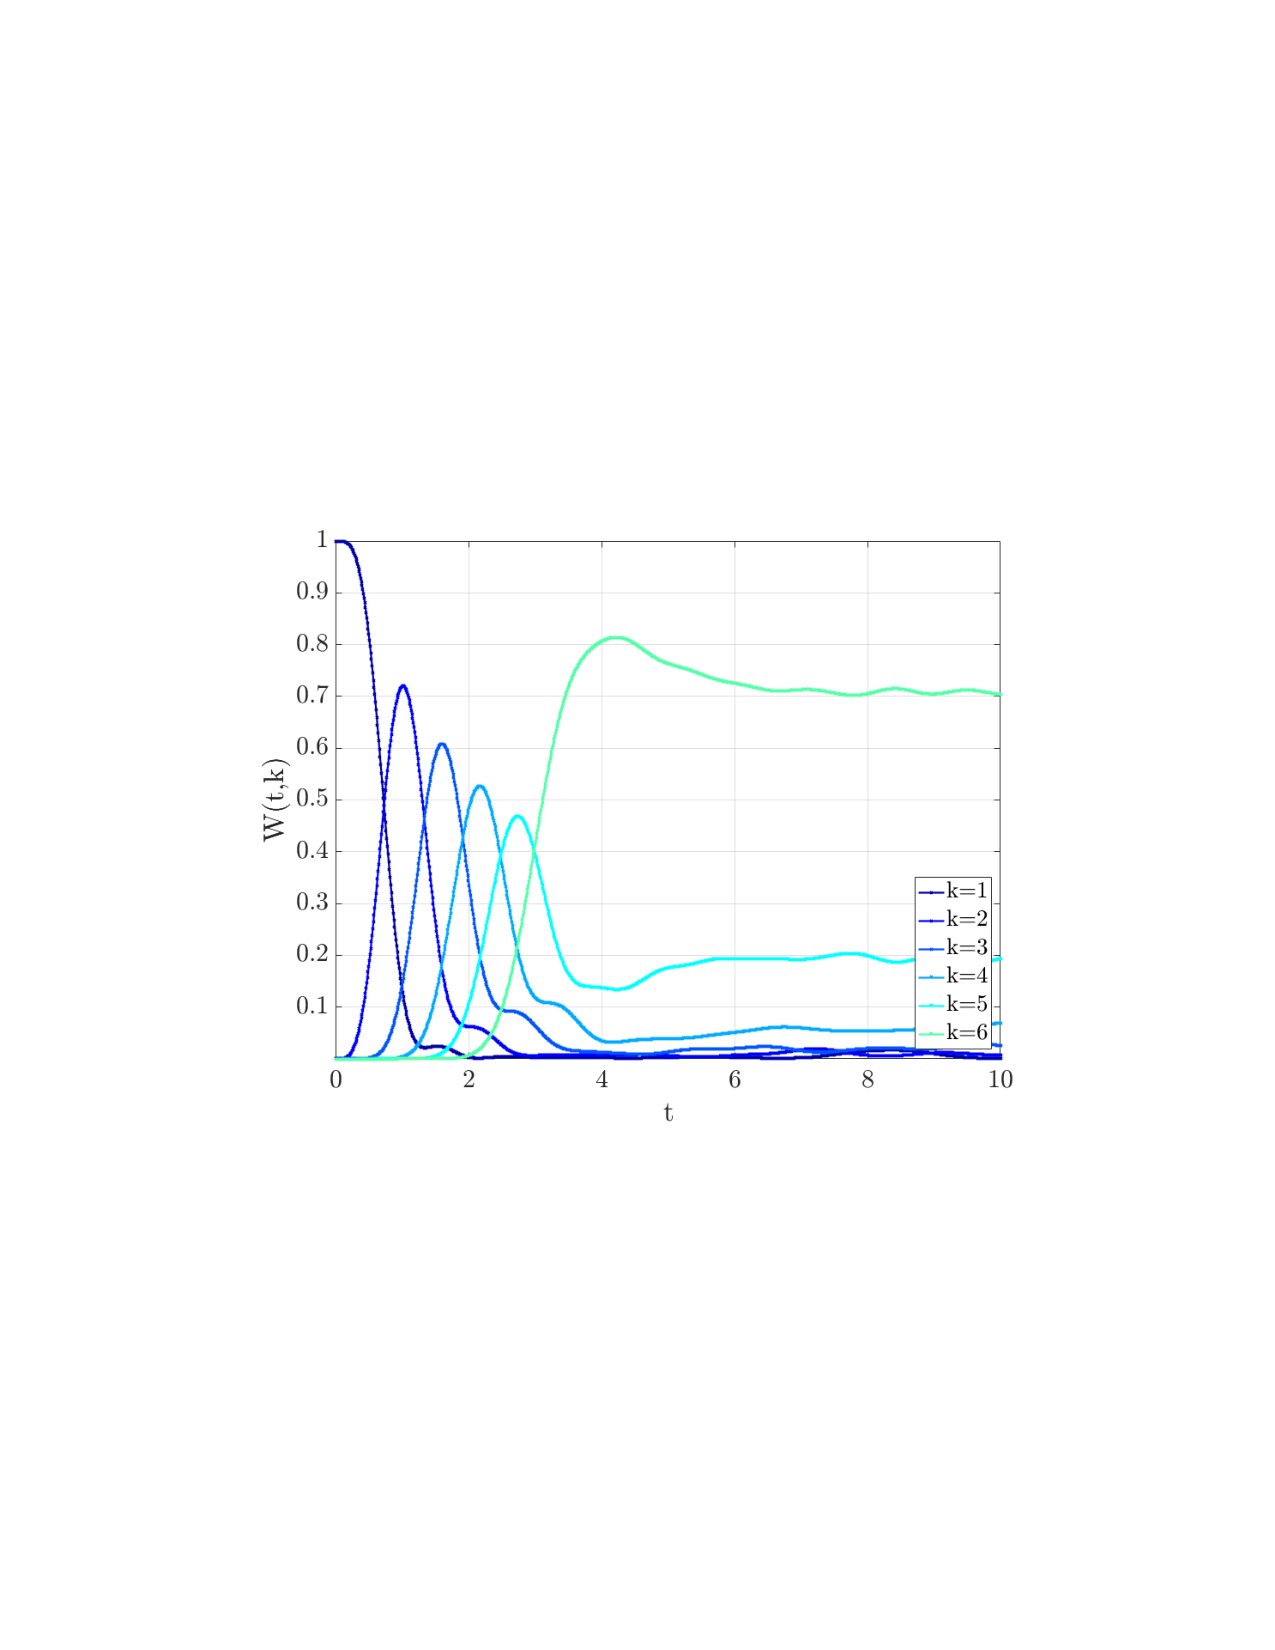
\includegraphics[width=.5\linewidth]{hamspreading}
	\caption{\textbf{Operator spreading as shown by the Pauli weight} in an Ising model with transverse field, from~\cite{Jonay17}. The end weight starts on site 1 and moves sequentially across the system to site 6. Note that the weights at any time sum to 1.}
	\label{fig:hamspreading}
\end{figure}

The Pauli decomposition is related to the Out-of-Time-Ordered Commutator (OTOC). Consider an initial operator, say, $A_0=Z_0=ZII\dots$, where the subscript now indicates that the operators on other sites are identities. This will commute with probe operators that are local at other sites, $B_i$. However, in general the time-evolved $A_0(t)$ will include Pauli strings that have non-identity operators at sire $i$. This can be seen through the Baker-Campbell-Hausdorff expansion~\cite{Roberts2016} of the time evolution
\begin{align}
A_0(t) &= \e^{iHt}A_0\e^{-iHt} \nn
&= \sum_k\frac{(it)^k}{k!}[H,[H,\dots[H,A_0]\dots]],\label{eqn:BCH}
\end{align}
where the dots represent that there are $k$ total commutators taken with $H$.
In general $H$ will contain matrix elements that connect the initially local operator to the non-local strings. Then, $A_0(t)$ can fail to commute with $B_i$, which is still local at $i$ and hasn't been evolved in time.

The extent to which these two fail to commute can be measured by the OTOC,\footnote{Should it be $1/q$ instead of $1/2$?}
\begin{align}
C(i,t) = \half\Tr \rho \abs{[A_0(t),B_i]}^2.\nonumber
\end{align}
For a pure state this is equivalent to~\cite{Keyserlingk, Jonay18}
\begin{align}
C(i,t) &= \half\langle\psi|\abs{[A_0(t),B_i]}^2|\psi\rangle\nn
&= 1-\Re\langle\psi|A_0(t)B_iA_0^\dag(t)B_i^\dag|\psi\rangle. \label{eqn:comm}
\end{align}
Some sources define the OTOC using $[A,B]^2$ instead of $|[A,B]|^2$~\cite{Jonay, Roberts2016, Nahum2017}. Others use the acronym to denote the out-of-time-order correlator, $F(i,t) = \ex{A_0(t)B_iA_0^\dag(t)B^\dag_i}$~\cite{Who}, which is related to $C(i,t)$ through Eq.~\ref{eqn:comm}. If $\rho$ is taken to be a thermal state at infinite temperature, the density matrix is proportional to the identity and the OTOC becomes
\begin{align}
C(i,t) = \half\Tr \abs{[A_0(t),B_i]}^2.
\end{align}
This definition can be thought of as independent of the state of the system. We will adopt this as our convention for the OTOC.

To see the relation between this quantity and $W(i,t)$, first consider the case of $q=2$. If the probe is $X_i$ there will be two classes of Pauli strings that commute with it: those with an identity at site $i$ and those with the operator $X$ at site $i$. Then $C(i,t)$ will be the sum of the squares of the $c_\mu(t)$ for which the operator at site $i$ is $Y$ or $Z$. If we average over choice of probe ($X$, $Y$, or $Z$), we arrive at 
\begin{align}
C(i,t) = \frac{2}{3}\sum_\nu|c_\nu(t)|^2\,\delta(\text{condition on $\nu$}),
	\label{eqn:otoc}
\end{align}
where the condition is that the operator at site $i$ is not the identity. For arbitrary $q$ the prefactor is $\frac{q^2-2}{q^2-1}$. 

If the operator $A_0(t)$ is sufficiently random, all $q^{2L}$ coefficients will have expectation values of the same order, with $|c_\nu|^2 \approx q^{-2L}$. There will be $q^{2L}\frac{q^2-1}{q^2}$ operators that meet the condition, so for these random operators
\begin{align}
C(i,t) &= \frac{q^2-2}{q^2-1}q^{2L}\frac{q^2-1}{q^2}\th{q^{2L}}\nn
&= \frac{q^2-2}{q^2}\nonumber.
\end{align}

For $q=2$ there is a particularly easy way to calculate the value in expression~\ref{eqn:otoc}. Since $\Tr(X) = \Tr(Y)=\Tr(Z) = 0$ and $\Tr(I) = 2$, in order to find the non-identity weight at site $i$ start by tracing over the degrees of freedom at that site to obtain $\tilde{A}_0(t) = \half\Tr_iA_0(t)$. Only the strings with the identity at $i$ survive this operation so
\begin{align}
\sum_\nu \abs{c_\nu(t)}^2\delta(\text{condition}) = \frac{3}{2}C(i,t) =  \Tr 
	\tilde{A}_0(t)\dag\tilde{A}_0(t).
\end{align}

\subsection{Information Velocities} \label{sub:vels}

Lieb-Robinson bounds

The butterfly velocity is the fastest velocity at which perturbations can propagate without decaying. In systems large enough so that the site index $i$ can be replaced with a continuous position $x$, the OTOC behaves as~\cite{Khemani2018}
\begin{align}
C(x,t)\sim \e^{\lambda(v)t}\quad\text{for}\;\;x=vt.\label{eqn:butterfly}
\end{align}
This tracks the OTOC along rays of constant velocity, as in Fig.~\ref{fig:khemani_lambda}.
\begin{figure}
	\centering
	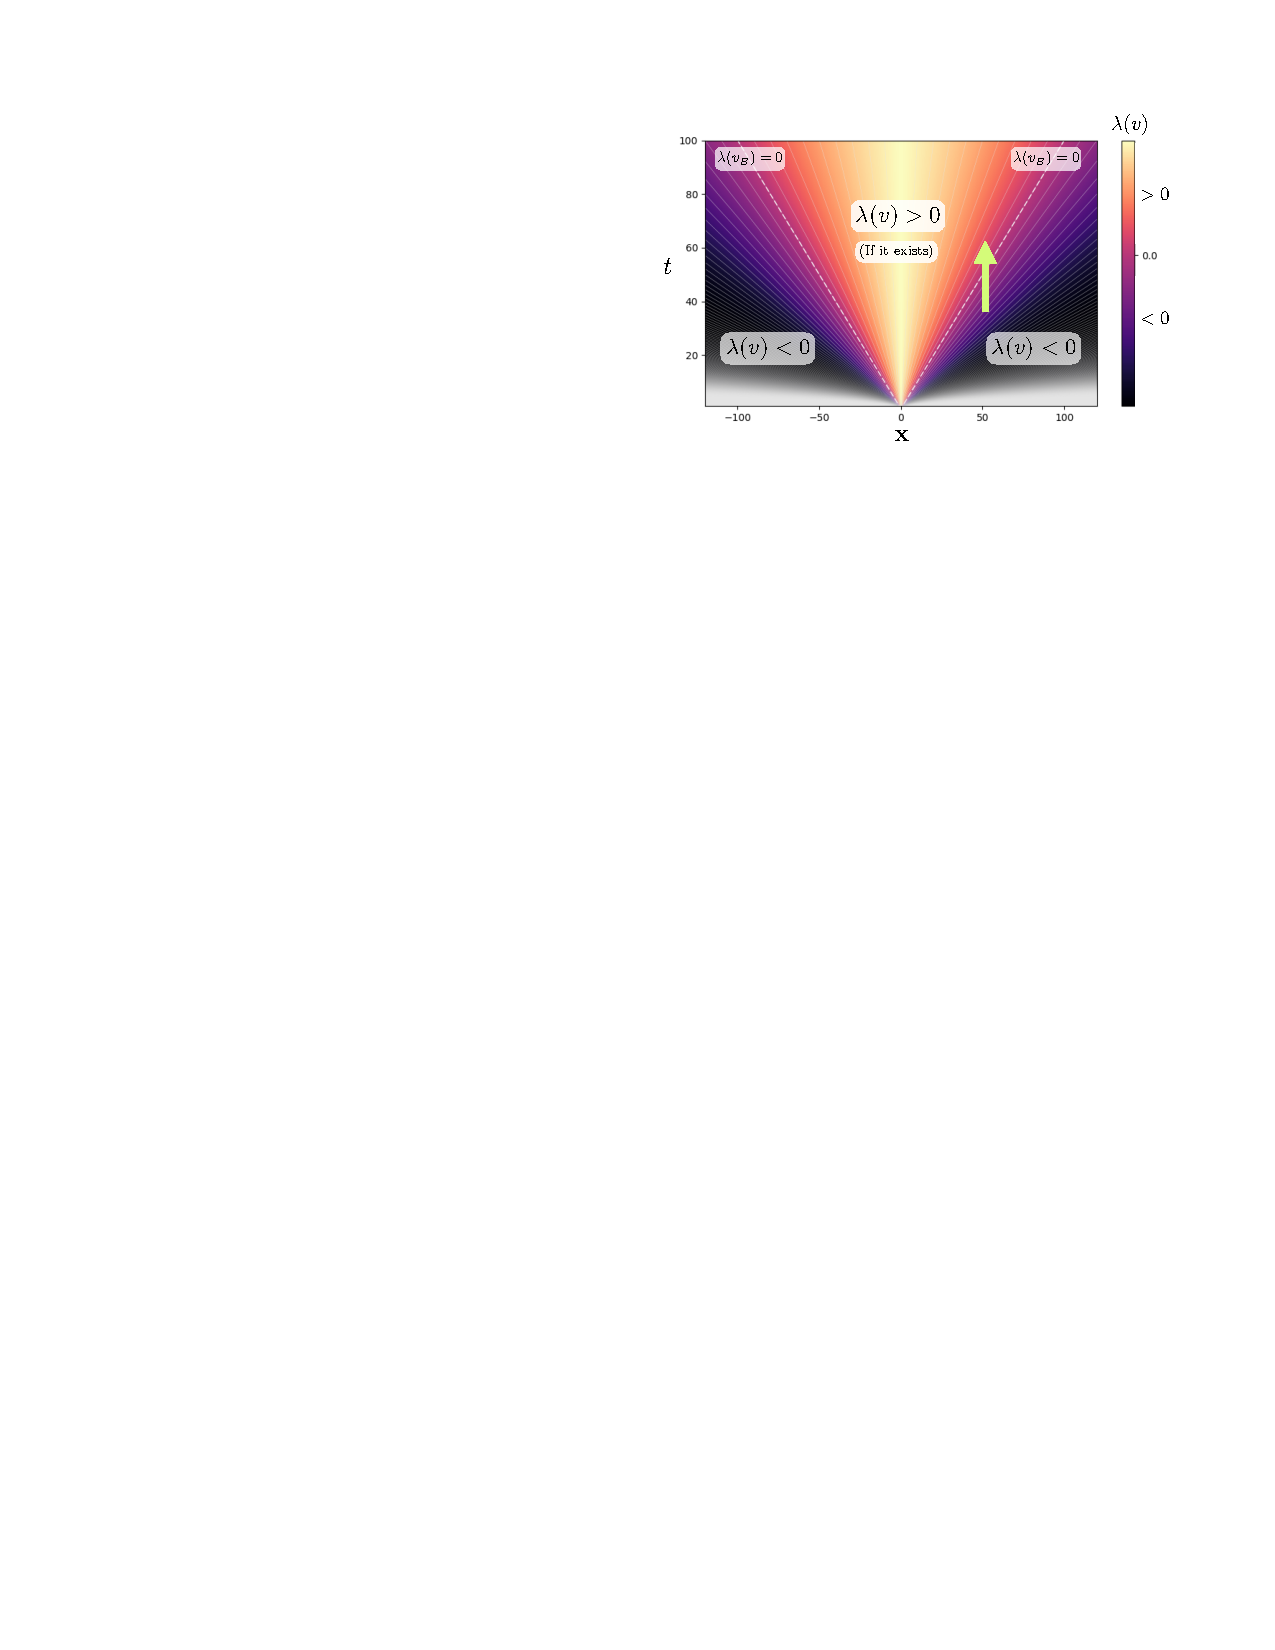
\includegraphics[width=.5\linewidth]{khemani_lambda}
	\caption{\textbf{Velocity dependent Lyapunov exponents} along rays of constant velocity, from~\cite{Khemani2018}. For $v<v_B$, inside the light cone, $\lambda>0$ or is not defined. Outside the light cone $\lambda<0$ and perturbations decay exponentially. The speed $v_B$ is where $\lambda=0$ and perturbations remain of order 1.}
	\label{fig:khemani_lambda}
\end{figure}
The fact that there is a single $v_B$ (or rather one in each direction) is due to the fact that $\lambda(v)$ must be convex, and can only cross 0 once.
